\section{Vehicle Ad-Hoc Networking (VANET)}
VANETs, which stands for Vehicular ad-hoc Network, is the idea of ad-hoc network communication between vehicles in real-time. Vehicles are able to communicate with other vehicles in their vicinity. VANETs is of interest to autonomous vehicles as valuable information may be shared within a linear road of autonomous vehicles. For example, the concept of platooning may be encouraged; autonomous vehicles are able to share acceleration or braking information for each instance of a vehicle so that all other vehicles behind are able to adjust accordingly so that vehicles driving along the road are in a train-like manner.

VANET models allow parking information shared from vehicle to vehicle within a vicinity. For example, when a car gives up a parking spot, it may announce as so, so that the information may be propagated to a car nearby looking for a space.

An increasing amount of vehicles are being equipped with on-board wireless communication units in order to facilitate wireless network among cars and their environments \citep{Lin2008SecurityNetworks}. Thus attention should be forwarded to simulate such a network with respect to smart parking functionalities.

In another VANET paper, the proposal brought forward involves a Voronoi diagram in order to dissect the regions of an urban area \citep{Panayappan2007VANET-basedAvailability}.

\begin{figure}[H]
    \centering
    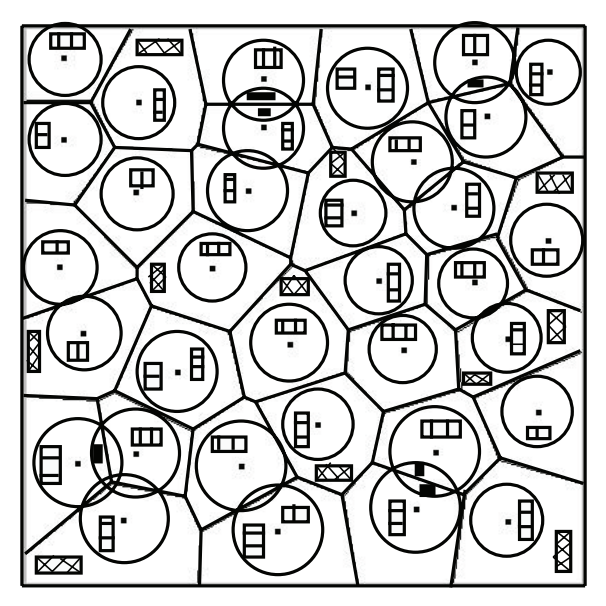
\includegraphics[width=0.5\linewidth]{./Images/VORONOI.png}
    \caption{Voronoi Model}
    \label{fig:sub1}
\end{figure}

Shown in fig. 1 is a Voronoi model dissecting each section of an urban area. The paper proposes that a road side unit (RSU) should be placed at the center of each individual sector; to handle all the information regarding parking information within its corresponding sector. Thus, each unit handles the occupancy levels of the parking spaces available to their designated areas and the cars with on-board wireless communications units may be able to communicate with each sector that it traverses through.

Although, the drawbacks with this type of implementation would be the cost, as the additional RSUs need to be deployed as well as parking sensors that monitor the parking spaces. This may be necessary for a VANET based system, however unlikely within an urban setting, there may be times where a vehicle is isolated from any nearby networks thus the lack of information for it would render it impossible to receive any type of information.

Furthermore, introduction of a VANET based system would also include distributed system models which have been researched much more thoroughly in terms of computer networks.